
\chapter{Proof techniques III --- Combinatorics}

\section{Counting}
\label{sec:counting}

\begin{enumerate}
\item Determine the number of entries in the following sequences.

  \begin{enumerate}
  \item \wbitemsep $(999, 1000, 1001, \ldots  2006)$
  \item \wbitemsep $(13, 15, 17, \ldots 199)$
  \item \wbitemsep $(13, 19, 25, \ldots 601)$
  \item \wbitemsep $(5, 10, 17, 26, 37, \ldots 122)$
  \item \wbitemsep $(27, 64, 125, 216, \ldots 8000)$
  \item \wbitemsep $(7, 11, 19, 35, 67, \ldots 131075)$
  \end{enumerate}

\workbookpagebreak

\item How many ``full houses'' are there in Yahtzee?  (A full house is a pair
together with a three-of-a-kind.)

\wbvfill

\item In how many ways can you get ``two pairs'' in Yahtzee?

\wbvfill

\item Prove that the binomial coefficients $\displaystyle \binom{n+k-1}{k}$
and $\displaystyle \binom{n+k-1}{n-1}$ are equal.

\wbvfill

\workbookpagebreak

\item The ``Cryptographer's alphabet'' is used to supply small examples
in coding and cryptography.  It consists of the first 6 letters, $\{a, b, c, d, e, f\}$.  How many ``words'' of length up to 6 can be made with this 
alphabet?  (A word need not actually be a word in English, for example 
both ``fed'' and ``dfe'' would be words in the sense we are using the term.)

\wbvfill

\item How many ``words'' are there of length 4, with distinct letters from the 
Cryptographer's alphabet, in which the letters appear in increasing order 
alphabetically?  (``Acef'' would be one such word, but ``cafe'' would not.)

\wbvfill

\item How many ``words'' are there of length 4 from the 
Cryptographer's alphabet, with repeated letters allowed,
 in which the letters appear in non-decreasing order alphabetically?

\wbvfill

\workbookpagebreak

\item How many subsets does a finite set have?

\wbvfill

\item How many handshakes will transpire when $n$ people first meet?

\wbvfill

\item How many functions are there from a set of size $n$ to a set of size $m$?

\wbvfill

\item How many relations are there from a set of size $n$ to a set of size $m$?

\wbvfill

\workbookpagebreak

\end{enumerate}

%% Emacs customization
%% 
%% Local Variables: ***
%% TeX-master: "GIAM-hw.tex" ***
%% comment-column:0 ***
%% comment-start: "%% "  ***
%% comment-end:"***" ***
%% End: ***



\clearpage

\section{Parity and Counting arguments}

\noindent{\large \bf Exercises --- \thesection\ }


\begin{enumerate}

\item A walking tour of K\"{o}nigsberg such as is described in this section,
or more generally, a circuit through an arbitrary graph that crosses each
edge precisely once and begins and ends at the same node is known as
an \index{Eulerian circuit} \emph{Eulerian circuit}.  An \index{Eulerian
path} \emph{Eulerian path} also crosses every edge of a graph exactly
once but it begins and ends at distinct nodes.  For each of the following
graphs determine whether an Eulerian circuit or path is possible, and if so,
draw it.

\begin{center}
\begin{picture}(0,0)%
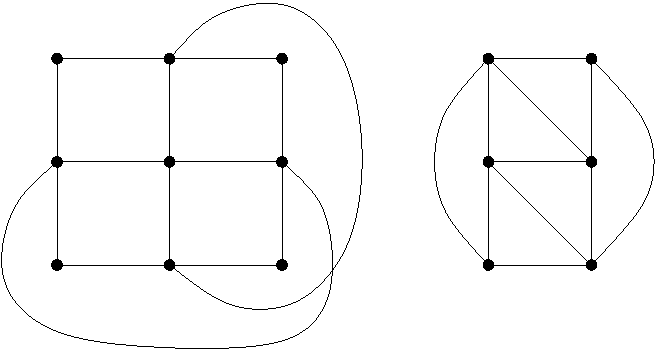
\includegraphics{./Euler_circuit_problems_a.pdf}%
\end{picture}%
\setlength{\unitlength}{3947sp}%
%
\begingroup\makeatletter\ifx\SetFigFont\undefined%
\gdef\SetFigFont#1#2#3#4#5{%
  \reset@font\fontsize{#1}{#2pt}%
  \fontfamily{#3}\fontseries{#4}\fontshape{#5}%
  \selectfont}%
\fi\endgroup%
\begin{picture}(5244,2786)(745,-2541)
\end{picture}%

\end{center}

\begin{center}
\begin{picture}(0,0)%
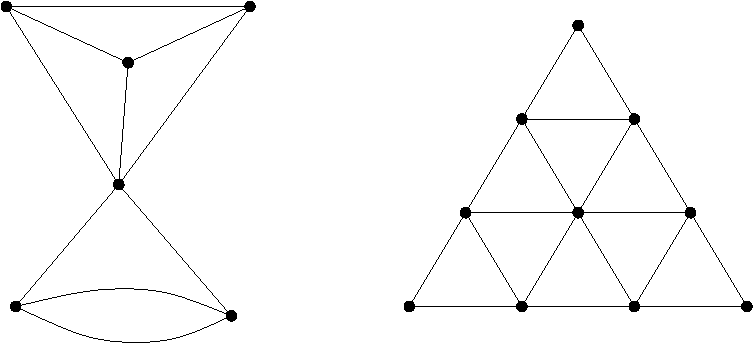
\includegraphics{./Euler_circuit_problems_b.pdf}%
\end{picture}%
\setlength{\unitlength}{3947sp}%
%
\begingroup\makeatletter\ifx\SetFigFont\undefined%
\gdef\SetFigFont#1#2#3#4#5{%
  \reset@font\fontsize{#1}{#2pt}%
  \fontfamily{#3}\fontseries{#4}\fontshape{#5}%
  \selectfont}%
\fi\endgroup%
\begin{picture}(6025,2749)(1226,-3136)
\end{picture}%

\end{center}

\item Complete the proof of the fact that ``Every graph has an even number
of odd nodes.''

\wbvfill

\item Provide an argument as to why an $8 \times 8$ chessboard with 
two squares pruned from diagonally opposite corners cannot be tiled
with dominoes.

\wbvfill

\workbookpagebreak

\item Prove that, if $n$ is odd, any $n \times n$ chessboard with 
a square the same color as one of its corners pruned can be tiled by
dominoes.

\wbvfill

\item The five \index{tetromino} tetrominoes (familiar to players of the video game
Tetris) are relatives of dominoes made up of four small squares.

\begin{center}
\begin{picture}(0,0)%
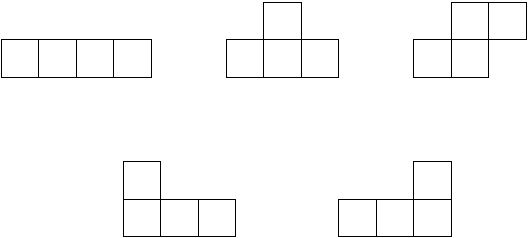
\includegraphics{figures/five_tetrominoes.pdf}%
\end{picture}%
\setlength{\unitlength}{3947sp}%
%
\begingroup\makeatletter\ifx\SetFigFont\undefined%
\gdef\SetFigFont#1#2#3#4#5{%
  \reset@font\fontsize{#1}{#2pt}%
  \fontfamily{#3}\fontseries{#4}\fontshape{#5}%
  \selectfont}%
\fi\endgroup%
\begin{picture}(4224,1899)(1189,-1948)
\end{picture}%

\end{center}

\noindent All together these five tetrominoes contain 20 squares
so it is conceivable that they could be used to tile a $4 \times 5$
chessboard.  Prove that this is actually impossible.

\wbvfill

\workbookpagebreak

\item State necessary and sufficient conditions for the existence of
an Eulerian circuit in a graph.  

\wbvfill

\item  State necessary and sufficient conditions for the existence of
an Eulerian path in a graph.  

\wbvfill

\newpage

\item Construct magic squares of order 4 and 5.

\wbvfill

\workbookpagebreak

\item A magic hexagon of order 2 would consist of filling-in
the numbers from 1 to 7 in the hexagonal array below.  The magic
condition means that each of the 9 ``lines'' of adjacent hexagons
would have the same sum.  Is this possible?

\begin{center}
\begin{picture}(0,0)%
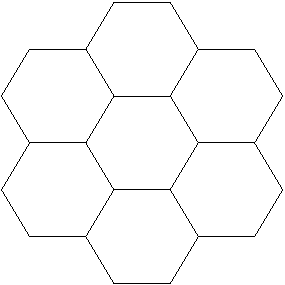
\includegraphics{figures/magic_hexagon.pdf}%
\end{picture}%
\setlength{\unitlength}{3947sp}%
%
\begingroup\makeatletter\ifx\SetFigFont\undefined%
\gdef\SetFigFont#1#2#3#4#5{%
  \reset@font\fontsize{#1}{#2pt}%
  \fontfamily{#3}\fontseries{#4}\fontshape{#5}%
  \selectfont}%
\fi\endgroup%
\begin{picture}(2274,2274)(2164,-3073)
\end{picture}%

\end{center}

\wbvfill

\item Is there a magic hexagon of order 3?

\wbvfill

\end{enumerate}



%% Emacs customization
%% 
%% Local Variables: ***
%% TeX-master: "GIAM-hw.tex" ***
%% comment-column:0 ***
%% comment-start: "%% "  ***
%% comment-end:"***" ***
%% End: ***



\clearpage


\section{The pigeonhole principle}

\noindent{\large \bf Exercises --- \thesection\ }

\begin{enumerate}

\item The statement that there are two non-bald New Yorkers with
the same number of hairs on their heads requires some careful 
estimates to justify it.  Please justify it.

\wbvfill

\item A mathematician, who always rises earlier than her spouse, has
developed a scheme -- using the pigeonhole principle -- to ensure that
she always has a matching pair of socks.  She keeps only blue socks, green 
socks and
black socks in her sock drawer -- 10 of each.  So as not to wake her 
husband she must
select some number of socks from her drawer in the early morning dark
and take them with her to the adjacent bathroom where she dresses.
What number of socks does she choose?

\wbvfill

\workbookpagebreak

\item If we select $1001$ numbers from the set $\{1, 2, 3, \ldots, 2000\}$
it is certain that there will be two numbers selected such that one divides
the other.  We can prove this fact by noting that every number in the given
set can be expressed in the form $2^k \cdot m$ where $m$ is an odd number
and using the pigeonhole principle.  Write-up this proof.

\wbvfill

\item Given any set of $53$ integers, show that there are two of them
having the property 
that either their sum or their difference is evenly divisible by $103$.

\wbvfill

\workbookpagebreak

\item Prove that if $10$ points are placed inside a square of side length 3,
there will be 2 points within $\sqrt{2}$ of one another.

\wbvfill

\item Prove that if $10$ points are placed inside an equilateral triangle
of side length 3, there will be 2 points within $1$ of one another.

\wbvfill

\workbookpagebreak

\item Prove that in a simple graph (an undirected graph with no 
loops or parallel edges) having $n$ nodes, there must be two nodes 
having the same degree. 

\wbvfill

\workbookpagebreak

\end{enumerate}


%% Emacs customization
%% 
%% Local Variables: ***
%% TeX-master: "GIAM-hw.tex" ***
%% comment-column:0 ***
%% comment-start: "%% "  ***
%% comment-end:"***" ***
%% End: ***



\clearpage

\section{The algebra of combinations}

\noindent{\large \bf Exercises --- \thesection\ }

\begin{enumerate}

\item Use the binomial theorem (with $x=1000$ and $y=1$) to calculate
$1001^6$.

\wbvfill

\item Find $(2x+3)^5$.

\wbvfill

\item Find $(x^2+y^2)^6$.

\wbvfill

\workbookpagebreak

\item The following diagram contains a 3-dimensional analog of
Pascal's triangle that we might call ``Pascal's tetrahedron.'' 
What would the next layer look like?

\begin{center}
\begin{picture}(0,0)%
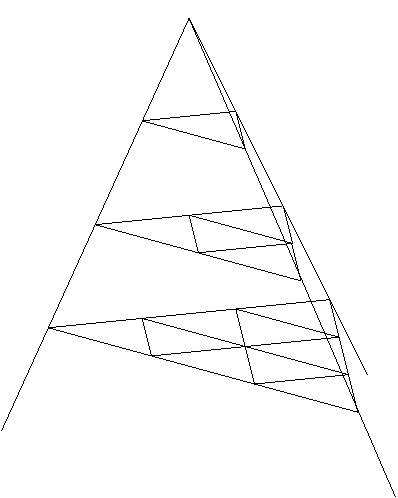
\includegraphics{figures/Pascals_tetrahedron.pdf}%
\end{picture}%
\setlength{\unitlength}{3947sp}%
%
\begingroup\makeatletter\ifx\SetFigFont\undefined%
\gdef\SetFigFont#1#2#3#4#5{%
  \reset@font\fontsize{#1}{#2pt}%
  \fontfamily{#3}\fontseries{#4}\fontshape{#5}%
  \selectfont}%
\fi\endgroup%
\begin{picture}(3174,3971)(3889,-4123)
\put(4876,-1111){\makebox(0,0)[lb]{\smash{{\SetFigFont{12}{14.4}{\familydefault}{\mddefault}{\updefault}{\color[rgb]{0,0,0}$1$}%
}}}}
\put(5851,-1036){\makebox(0,0)[lb]{\smash{{\SetFigFont{12}{14.4}{\familydefault}{\mddefault}{\updefault}{\color[rgb]{0,0,0}$1$}%
}}}}
\put(5926,-1411){\makebox(0,0)[lb]{\smash{{\SetFigFont{12}{14.4}{\familydefault}{\mddefault}{\updefault}{\color[rgb]{0,0,0}$1$}%
}}}}
\put(6526,-2536){\makebox(0,0)[lb]{\smash{{\SetFigFont{12}{14.4}{\familydefault}{\mddefault}{\updefault}{\color[rgb]{0,0,0}$1$}%
}}}}
\put(6226,-1786){\makebox(0,0)[lb]{\smash{{\SetFigFont{12}{14.4}{\familydefault}{\mddefault}{\updefault}{\color[rgb]{0,0,0}$1$}%
}}}}
\put(4501,-1936){\makebox(0,0)[lb]{\smash{{\SetFigFont{12}{14.4}{\familydefault}{\mddefault}{\updefault}{\color[rgb]{0,0,0}$1$}%
}}}}
\put(4135,-2779){\makebox(0,0)[lb]{\smash{{\SetFigFont{12}{14.4}{\familydefault}{\mddefault}{\updefault}{\color[rgb]{0,0,0}$1$}%
}}}}
\put(4955,-2642){\makebox(0,0)[lb]{\smash{{\SetFigFont{12}{14.4}{\familydefault}{\mddefault}{\updefault}{\color[rgb]{0,0,0}$3$}%
}}}}
\put(5719,-2580){\makebox(0,0)[lb]{\smash{{\SetFigFont{12}{14.4}{\familydefault}{\mddefault}{\updefault}{\color[rgb]{0,0,0}$3$}%
}}}}
\put(6631,-2841){\makebox(0,0)[lb]{\smash{{\SetFigFont{12}{14.4}{\familydefault}{\mddefault}{\updefault}{\color[rgb]{0,0,0}$3$}%
}}}}
\put(6720,-3140){\makebox(0,0)[lb]{\smash{{\SetFigFont{12}{14.4}{\familydefault}{\mddefault}{\updefault}{\color[rgb]{0,0,0}$3$}%
}}}}
\put(6782,-3494){\makebox(0,0)[lb]{\smash{{\SetFigFont{12}{14.4}{\familydefault}{\mddefault}{\updefault}{\color[rgb]{0,0,0}$1$}%
}}}}
\put(5861,-3409){\makebox(0,0)[lb]{\smash{{\SetFigFont{12}{14.4}{\familydefault}{\mddefault}{\updefault}{\color[rgb]{0,0,0}$3$}%
}}}}
\put(5026,-3184){\makebox(0,0)[lb]{\smash{{\SetFigFont{12}{14.4}{\familydefault}{\mddefault}{\updefault}{\color[rgb]{0,0,0}$3$}%
}}}}
\put(5866,-2894){\makebox(0,0)[lb]{\smash{{\SetFigFont{12}{14.4}{\familydefault}{\mddefault}{\updefault}{\color[rgb]{0,0,0}$6$}%
}}}}
\put(6319,-2377){\makebox(0,0)[lb]{\smash{{\SetFigFont{12}{14.4}{\familydefault}{\mddefault}{\updefault}{\color[rgb]{0,0,0}$1$}%
}}}}
\put(6271,-2102){\makebox(0,0)[lb]{\smash{{\SetFigFont{12}{14.4}{\familydefault}{\mddefault}{\updefault}{\color[rgb]{0,0,0}$2$}%
}}}}
\put(5330,-1817){\makebox(0,0)[lb]{\smash{{\SetFigFont{12}{14.4}{\familydefault}{\mddefault}{\updefault}{\color[rgb]{0,0,0}$2$}%
}}}}
\put(5406,-2329){\makebox(0,0)[lb]{\smash{{\SetFigFont{12}{14.4}{\familydefault}{\mddefault}{\updefault}{\color[rgb]{0,0,0}$2$}%
}}}}
\put(5441,-299){\makebox(0,0)[lb]{\smash{{\SetFigFont{12}{14.4}{\familydefault}{\mddefault}{\updefault}{\color[rgb]{0,0,0}$1$}%
}}}}
\end{picture}%

\end{center}

\wbvfill

\item The student government at Lagrange High consists of 24 members chosen
from amongst the general student body of 210. Additionally, there
is a steering committee of 5 members chosen from amongst those in
student government. Use the multiplication rule to determine two different
formulas for the total number of possible governance structures.

\wbvfill

\workbookpagebreak

\item Prove the identity
\[ \binom{n}{k} \cdot \binom{k}{r} \; = \; \binom{n}{r} \cdot \binom{n-r}{k-r} \]
combinatorially.

\wbvfill

\item Prove the binomial theorem.

\[ \forall n \in \Naturals, \; \forall x,y \in \Reals, \; 
(x+y)^n \; = \; \sum_{k=0}^n \binom{n}{k} x^{n-k}y^k \]

\wbvfill

\workbookpagebreak

\end{enumerate}

%% Emacs customization
%% 
%% Local Variables: ***
%% TeX-master: "GIAM-hw.tex" ***
%% comment-column:0 ***
%% comment-start: "%% "  ***
%% comment-end:"***" ***
%% End: ***




%% Emacs customization
%% 
%% Local Variables: ***
%% TeX-master: "GIAM-hw.tex" ***
%% comment-column:0 ***
%% comment-start: "%% "  ***
%% comment-end:"***" ***
%% End: ***

